\chapter{MixVRTの実装}\label{cha:Implementation}
本章では、\toolName の実装について説明する。
\toolName のシステム構成(仮)を、図\ref{fig:System}に示す。
\begin{figure}[tp]
    \begin{center}
        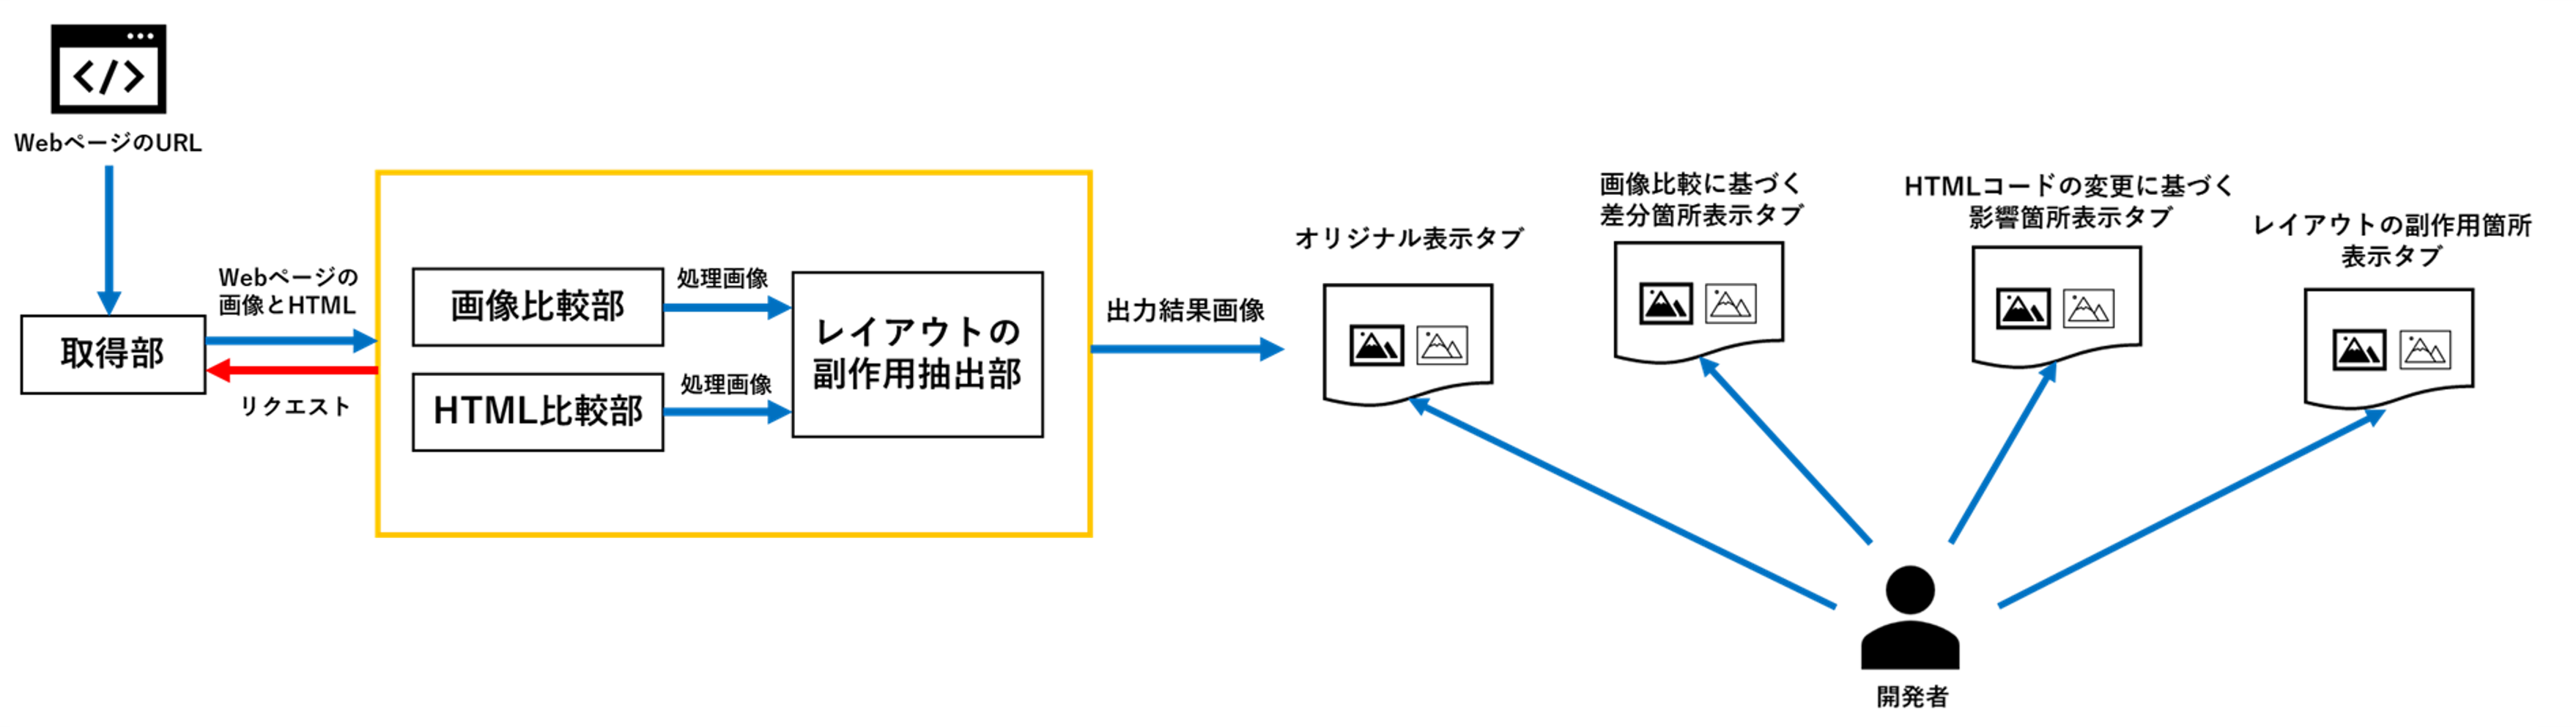
\includegraphics[width=1.0\columnwidth]{image/4_System.png}
        \caption{\toolName のシステム構成(仮)}
        \label{fig:System}
    \end{center}
\end{figure}
% 私の開発したツールは、まずユーザーがWebページのURLを入力します。
% このURLを受け取ると、ツールは該当するWebページから画像を取得し、
% これらの画像に対して特定の処理を行います。処理された画像は"static/images"ディレクトリに保存されます。
% そして、Flaskがローカルサーバを提供し、
% "templates"フォルダにあるHTMLファイルが"static/images"ディレクトリを参照できるようになっています。
% この仕組みにより、ユーザーはローカルに立てられたFlaskサーバを通じて、
% Webページ上で生成された画像を確認することができます。
本研究では、\toolName の試作にあたり、以下の5つの処理部を実装する。
\begin{itemize}
    \item Webデータ取得部
    \item 画像比較部
          \begin{enumerate}
              \item 差分箇所検出
              \item 差分箇所枠抽出
          \end{enumerate}
    \item HTML比較部
          \begin{enumerate}
              \item 差分ファイル生成
              \item 差分ファイル解析
              \item 影響箇所強調HTMLコード生成
              \item 影響箇所枠抽出
          \end{enumerate}
    \item レイアウトの副作用箇所抽出部
    \item インターフェース表示部
\end{itemize}
% \begin{itemize}
%     \item Webデータ取得部
%     \item 画像比較部
%           \begin{enumerate}
%               \item 差分箇所検出
%           \end{enumerate}
%     \item HTML比較部
%           \begin{enumerate}
%               \item 差分ファイル生成
%               \item 差分ファイル解析
%               \item 影響箇所強調HTMLコード生成
%           \end{enumerate}
%     \item レイアウトの副作用箇所抽出部
%     \item インターフェース表示部
% \end{itemize}
以降、\toolName を構成する5つの処理部について説明する。
\par

\section{Webデータ取得部}\label{sec:Web_data_get_section}
Webデータ取得部は、WebページのURLを入力として受け取り、Webページの画像とHTMLコードを取得する。
取得したWebページの画像は画像比較部(\ref{sec:Difference_extraction_section}節で後述)に出力し、取得したWebページのHTMLコードはHTML比較部(\ref{sec:Affected_area_extraction}節で後述)に出力する。
なお、HTML比較部がWebデータ取得部にWebページのURLを与えて呼び出す場合においては、Webページの画像のみをHTML比較部に出力する。
Webページの画像取得には、Selenium WebDriver(\ref{sec:Selenium_WebDriver}節を参照)を用いてWebページの画像を取得する。
Selenium WebDriverを用いて取得したWebページの画像例を、図\ref{fig:4_get_images}に示す。
\begin{figure}[tp]
    \begin{center}
        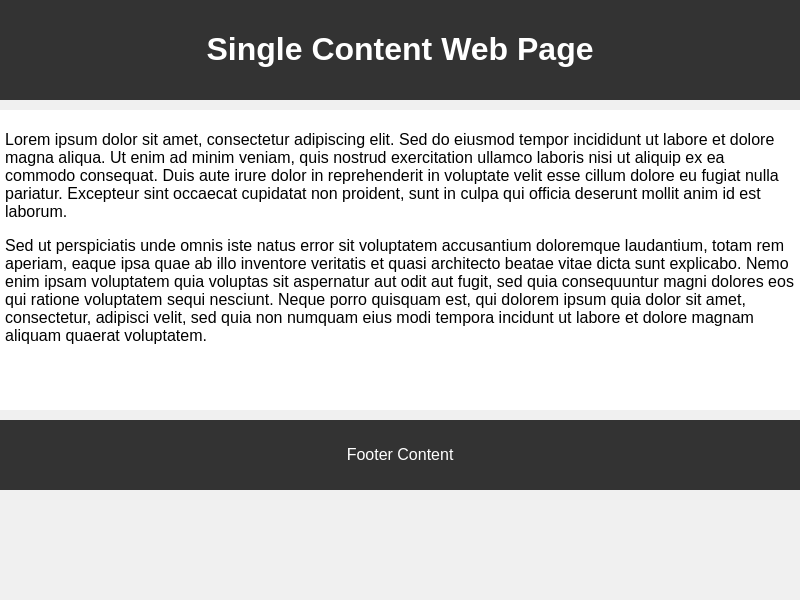
\includegraphics[width=1.0\columnwidth]{image/4_get_images.png}
        \caption{Selenium WebDriverを用いて取得したWebページの画像例}
        \label{fig:4_get_images}
    \end{center}
\end{figure}
WebページのHTMLコード取得には、Pythonライブラリの一つであるrequestsモジュール(\ref{sec:requests}節を参照)を用いて、WebページのURLからWebページのHTMLコードを取得する。
requestsモジュールを用いて取得したWebページのHTMLコード例を、ソースコード\ref{lst:html_example}に示す。
\begin{lstlisting}[language=HTML, caption=requestsモジュールを用いて取得したWebページのHTMLコード例, label=lst:html_example]
    <!DOCTYPE html>
    <html lang="en">
    
    <head>
        <meta charset="UTF-8">
        <meta name="viewport" content="width=device-width, initial-scale=1.0">
        <title>Single Content Web Page</title>
        <style>
            body {
                font-family: Arial, sans-serif;
                margin: 0;
                padding: 0;
                background-color: #f0f0f0;
            }
    
            header {
                background-color: #333;
                color: white;
                text-align: center;
                padding: 10px 0;
            }
    
            .container {
                height: 300px auto;
                width: 100%;
                margin: 10px auto;
                overflow: hidden;
            }
    
            .main-content {
                height: 300px;
                background-color: #fff;
                padding: 5px;
                box-sizing: border-box;
            }
    
            footer {
                background-color: #333;
                color: white;
                text-align: center;
                padding: 10px 0;
                clear: both;
            }
        </style>
    </head>
    
    <body>
        <header>
            <h1>Single Content Web Page</h1>
        </header>
        <div class="container">
            <div class="main-content">
                <p>Lorem ipsum dolor sit amet, consectetur adipiscing elit. Sed do eiusmod tempor incididunt ut labore et
                    dolore magna aliqua. Ut enim ad minim veniam, quis nostrud exercitation ullamco laboris nisi ut aliquip
                    ex ea commodo consequat. Duis aute irure dolor in reprehenderit in voluptate velit esse cillum dolore eu
                    fugiat nulla pariatur. Excepteur sint occaecat cupidatat non proident, sunt in culpa qui officia
                    deserunt mollit anim id est laborum.</p>
                <p>Sed ut perspiciatis unde omnis iste natus error sit voluptatem accusantium doloremque laudantium, totam
                    rem aperiam, eaque ipsa quae ab illo inventore veritatis et quasi architecto beatae vitae dicta sunt
                    explicabo. Nemo enim ipsam voluptatem quia voluptas sit aspernatur aut odit aut fugit, sed quia
                    consequuntur magni dolores eos qui ratione voluptatem sequi nesciunt. Neque porro quisquam est, qui
                    dolorem ipsum quia dolor sit amet, consectetur, adipisci velit, sed quia non numquam eius modi tempora
                    incidunt ut labore et dolore magnam aliquam quaerat voluptatem.</p>
            </div>
        </div>
        <footer>
            <p>Footer Content</p>
        </footer>
    </body>
    
    </html>
\end{lstlisting}

\section{差分箇所検出部}\label{sec:Difference_extraction_section}
差分箇所検出部は、Webページ情報取得部からWebページの画像を受け取り、差分箇所を色付きの枠で囲んで強調表示した画像を生成する。
PythonのOpenCV\cite{OpenCV}を用いた差分箇所検出の手順を以下に示す。
\begin{enumerate}
    \item 高解像度画像生成処理
    \item 適応的二値化処理
    \item 差分検出処理
    \item 膨張処理
    \item 輪郭検出処理
    \item バウンディングボックス描画処理
\end{enumerate}

\subsection{高解像度画像生成処理}\label{subsec:Generate_high_images}
高解像度画像生成処理は、元のWebページ画像をもとに高解像度画像を生成する。高解像度画像は、輪郭検出処理(\ref{subsec:contour_detection_processing}で後述)の精度を向上するために必要である。
具体的な処理手順を、以下に示す。

元のWebページ画像はpng画像であり、png画像をsvgファイルに変換し、さらにsvgファイルをpdfファイルに変換した後、pdfファイルをpng画像に戻す処理を行うことで、高解像度のpng画像を生成することができる。
まず、png画像をsvg画像に変換するには、Aspose.Wordsライブラリのaw.Document()とaw.DocumentBuilder()を使用して、png画像をドキュメントに挿入し、Aspose.WordsのImageSaveOptionsを使用して、画像をsvg形式で保存する。
次に、svg画像からpdf画像に変換するには、svglibとreportlabライブラリを使用して、svgファイルをpdfファイルに変換する。
最後にpdfファイルからpng画像に変換するには、pdf2imageライブラリのconvert\_from\_path関数を使用して、pdfファイルをpng画像に変換する。この際、解像度を300DPI(Dots Per Inch:1インチ当たりのドット数)に設定することで、
150DPI(Dots Per Inch)である元のWebページ画像の2倍解像度が高解像度画像を生成する。

% アンダーバー"_"は"\"でエスケープする

\subsection{適応的二値化処理}\label{subsec:Adaptive_Binarisation}
適応的二値化処理は、Webページの画像の二値化(白黒化)を行う。
Webページの画像を二値化する流れを、以下に示す。
\begin{enumerate}
    \item OpenCVのimread関数を用いて、Webページの画像パスから画像を読み込む。
    \item OpenCVのcvtColor関数を用いて、画像をグレースケール化する。
    \item OpenCVのadaptiveThreshold関数を用いて、画像の二値化を行う。
\end{enumerate}


\subsection{差分検出処理}\label{subsec:difference_detection_process}
OpenCVのsubtract関数を用いて、Webページの変更前画像で削除された箇所とWebページの変更後画像で追加された箇所を検出する。

\subsection{膨張処理}\label{subsec:dilation}
膨張処理をすることで、大体の大枠で差分を検出できるようにする。

\subsection{輪郭検出処理}\label{subsec:contour_detection_processing}
差分検出処理で検出した差分を枠で囲むような輪郭を検出する。画面要素はある程度他の画面要素と離れて独立しているため、大体で差分箇所の場所を示すことができる。画面要素単位で差分を検出するために膨張処理を行った。

\subsection{バウンディングボックス描画処理}\label{subsec:Bounding box drawing process}
バウンディングボックス描画処理では、元画像に輪郭検出処理で検出した枠を描画する。


\section{影響箇所検出部}\label{sec:Affected_area_extraction}
HTMLコードの変更に基づく影響箇所抽出部は、Webページ情報取得部で取得した変更前後のWebページのHTMLコードを用いて影響箇所を特定する。
概要としては、差分ファイルを生成し、差分ファイルから枠付け処理を行った変更前後のHTMLコードを生成した後、そのHTMLコードをFlaskのテンプレートエンジンを用いてWebページを表示し、Webページ情報取得部によってそのWebページの画像を取得する。
元のWebページ画像と枠付け処理をしたWebページ画像を比較して枠のみを抽出する。
具体的には、まず、Pythonライブラリの一つであるdifflibモジュールを用いて、変更前後のHTMLコードから差分ファイルを生成する。
生成した差分ファイルは、コードの追加行には"+", 削除行には"-", 変更前後のHTMLコードにどちらにも存在しない行には"?"が先頭に付き、"?"を除いた差分ファイルを解析対象とする。
差分ファイルは、bodyタグ内とstyleタグ内を対象とする。
もし、bodyタグ内で先頭に"+"や"-"があれば、コードの追加や削除、変更があったとして、その箇所に枠付け処理を行うCSSクラスを追加し、先頭の"+"か"-"を削除する。
styleタグ内の場合は、CSSクラスのセレクタ名のみの変更やスタイルのみの変更、またはその両方の変更があったCSSクラスを対象として、そのCSSクラスに対して枠付けを行うスタイルを適用する。
この場合においても、解析した行の先頭に"+", "-"があれば削除する。
差分ファイルから枠付け処理を行った変更前後のHTMLコードを生成した後は、そのHTMLコードをFlaskのテンプレートエンジンを用いてWebページとして表示し、そのWebページの画像を取得する。
そして、元のWebページ画像と枠付け処理をしたWebページ画像を比較して枠のみを抽出する。

\section{レイアウトの副作用箇所抽出部}\label{sec:Layout_subEffect_extraction_section}
レイアウトの副作用箇所抽出部は、画像比較に基づく差分箇所とHTMLコードの変更に基づく影響箇所を用いて、レイアウトの副作用箇所を抽出する。
具体的には、差分箇所を囲む枠と影響箇所を囲む枠同士を比較する。比較の仕方は、枠の重なり度合を判定する。
まず、枠が重なっているかどうかを判定する。次に、枠が重なっている場合に、重なり部分が小さい方の枠の面積の6割以上であれば枠が一致すると判定する。
最終的に、一致しない枠のみを抽出し、Webページの元画像に描画する。


\section{インターフェース表示部}\label{sec:Interface_Display_Section}
インターフェース表示部は、\ref{sec:Web_data_get_section}節~\ref{sec:Layout_subEffect_extraction_section}節で取得・生成した画像(枠強調マスク画像を除く)を保管し、Webベースのユーザインターフェースを用いて表示する。
MixVRTの実行コマンド初回実行時は、\ref{sec:Web_data_get_section}節で取得したWebページの画像を保管する。
MixVRTの実行コマンド2回目以降実行時は、初回実行時に取得する画像に加えて、\ref{sec:Difference_extraction_section}節で取得した画像、
\ref{sec:Affected_area_extraction}節で生成した画像、\ref{sec:Layout_subEffect_extraction_section}節で生成した画像を保管する。



% \section{画像とHTMLコード取得部}\label{sec:area_detection_part}

% \subsection{Seleniumによる画像取得}\label{subsec:rect_detection}

% \subsection{requestsによるHTMLコード取得}\label{subsec:underline_detection}


% \section{差分抽出部}\label{sec:OCR_part}

% \subsection{画像比較による差分抽出}\label{subsec:char_extraction}

% \subsection{HTMLの変更による影響箇所抽出}\label{subsec:bbox_coords_obtainment}

% \subsection{画像とHTMLコードに基づくレイアウトの副作用抽出}\label{subsec:bbox_obtainment}


% \section{差分表示部}\label{sec:label_link_part}